\section{Introduction}

Recently, Linux containers have drawn significant amount of attention because they are lightweight, portable, and repeatable.
Linux containers are generally more lightweight than virtual machine (VM) clusters, 
because the containers share the kernel with the host operating system (OS), even though they maintain separate execution environments. 
They are generally portable because the process execution environments are archived into tar files, 
so whenever one attempts to run a container, the exact same file systems are restored from the archives 
even when totally different data centers are used. 
This means that containers can provide repeatable and portable execution environments.
%
For the same reasons, Linux containers are attractive for web services as well, 
and it is expected that web services consisting of container clusters would be 
capable of being migrated easily for variety of purposes. For example disaster recovery, 
cost performance improvemets, legal compliance, and shortening the geographical distance to customers 
are the main concerns for web service providers in e-commece, gaming, Financial technology(Fintech) and Internet of Things(IoT) field.
%

Kubernetes\cite{K8s2017}, which is one of the popular container cluster management systems, 
enables easy deployment of container clusters.
Since Kubernetes hides the differences in the base environments, users can easily deploy a web service on different 
cloud providers or on on-premise data centers, without adjusting the container cluster configurations to the new environment. 
This allows a user to easily migrate a web service consisting of a container cluster even to the other side of the world. 
A user starts the container cluster in the new location, route the traffic there, 
then stop the old container cluster at his or her convenience.
This is a typical web service migration scenario.

However, this scenario only works when the user migrates a container cluster among major cloud providers including Google Cloud Platform (GCP), 
Amazon Web Services (AWS), and Microsoft Azure.
The Kubernetes does not include a load balancer, and is heavily dependent on external load balancers that are set up on the fly 
by cloud providers through their application protocol interfaces (APIs). 
These external load balancers distribute incoming traffic to every server that hosts containers.
The traffic is then distributed again to destination containers using iptables destination 
network address translation (DNAT)\cite{MartinA.Brown2017,Marmol2015} rules in a round-robin manner. 
The problem happens in the environment with a load balancer that is not supported by the Kubernetes, 
e.g. in an on-premise data center with a bare metal load balancer. 
In such environments, the user needs to manually configure 
the static route for inbound traffic in an ad-hoc manner. 
Since the Kubernetes fails to provide an uniform environment from a container cluster view point,
migrating container clusters among the different environments will always be a burden.

In order to solve this problem by eliminating the dependency on external load balancer,
herein we propose a containerized software load balancer that is run by Kubernetes as  
as a part of web services consisting of container cluster.
It enables a user to easily deploy a web service on different environment without modification, 
because the load balancer is included in the web service itself. 
To accomplish this, we will containerize Linux kernel's Internet Protocol Virtual Server (IPVS)\cite{Zhang2000} 
Layer 4 load balancer using an existing Kubernetes ingress\cite{K8sIngress2017} framework, as a proof of concept.
%
%
To prove that our approach will not significantly deteriorate the performance,  
we will also compare the performance of our proposed load balancer with those of 
iptables DNAT load balancer and the Nginx Layer 7 load balancing. 
%
The results indicated that the proposed load balancer could improve the portability of container clusters 
without performance degradation compared with the existing load balancer.
The performance of the proposed load balancer may be affected by the network configurations of overlay network 
and distributed packet processing. 
We also evaluate how the network configurations affects the performance and discusses 
the best setting that derives the best performance.

The contributions of this paper are as follows: 
1) We propose a portable software load balancer that is runnable on any cloud provider, or on on-premise data centers, 
as a part of a container cluster.
2) We discuss feasibility of the proposed load balancer by comparing its performance with other load balancers.
3) We also discuss usable overlay network configurations and clarify the importance of techniques 
that will  draw the best performance from such load balancers.  

The rest of the paper is organized as follows.
Section \ref{Related Work} highlights work that deals specifically with container cluster migration, 
software load balancer containerization, and load balancer related tools within the context of the container technology. 
Section \ref{Load balancers in Kubernetes cluster} will explain existing architecture problems and propose our solutions.
In Section \ref{Performance Measurement}, experimental conditions and the parameters 
that we considered to be important in our experiment will be described in detail.
Then, we will show our experimental results and discuss the obtained performance characteristics in Section~\ref{Result and Discussion},  
which is followed by a summary of our work in Section~\ref{Conclusions}.

\section{Related Work}\label{Related Work}

This section highlights related work, especially that dealing with container cluster migration, 
software load balancer containerization, and load balancer tools within the context of the container technology.

\paragraph{\bf Container cluster migration:}

Kubernetes developers are trying to add federation\cite{K8sFederation2017} capability for handling situations 
where multiple Kubernetes clusters\footnote{The {\em Kubernetes cluster} refers to a server cluster 
controlled by the Kubernetes container management system, in this paper.} 
are deployed on multiple cloud providers or on-premise data centers, 
and are managed via the Kubernetes federation API server (federation-apiserver). 
However, how each Kubernetes cluster is run on different types of cloud providers
and/or on-premise data centers, especially when the load balancers of such environments are not supported by Kubernetes, 
seems beyond the scope of that project. 
The main scope of this paper is to make Kubernetes usable in environments 
without supported load balancers by providing a containerized software load balancer.

\paragraph{\bf Software load balancer containerization:}
As far as load balancer containerization is concerned, the following related work has been identified:
Nginx-ingress\cite{Pleshakov2016,NginxInc2016} utilizes the ingress\cite{K8sIngress2017} capability of Kubernetes, 
to implement containerized Nginx proxy as a load balancer. Nginx itself is famous as a high-performance web server program
that also has the functionality of a Layer-7 load balancer. Nginx is capable of handling Transport Layer Security(TLS) encryption, 
as well as Uniform Resource Identifier(URI) based switching. However, the flip side of Nginx is that it is much slower than Layer-4 switching.
We compared the performance between Nginx as a load balancer and our proposed load balancer in this paper.
%
Meanwhile, the kube-keepalived-vip\cite{Prashanth2016} project is trying to use Linux kernel's IPVS\cite{Zhang2000} 
load balancer capabilities by containerizing the keepalived\cite{ACassen2016}.
The kernel IPVS function is set up in the host OS's net name spaces and is shared among multiple web services,
as if it is part of the Kubernetes cluster infrastructure.
Our approach differs in that the IPVS rules are set up in container's net name spaces 
and function as a part of the web service container cluster itself.
The load balancers are configurable one by one, and are  movable with the cluster once the migration is needed.
The kube-keepalived-vip's approach lacks flexibility and portability whereas ours provide them.
%
The swarm mode of the Docker\cite{DockerCoreEngineering2016,DockerInc2017} also uses IPVS for internal load balancing,
but it is also considered as part of Docker swarm infrastructure, 
and thus lacks the portability that our proposal aims to provide.

\paragraph{\bf Load balancer tools in the container context:}
There are several other projects where efforts have been made to utilize IPVS in the context of container environment.
For example, GORB\cite{Sibiryov2015} and clusterf\cite{Aaltodoc:http://urn.fi/URN:NBN:fi:aalto-201611025433} are daemons 
that setup IPVS rules in the kernel inside the Docker container. 
They utilize running container information stored in key-value storages
like Core OS etcd\cite{CoreOSEtcd} and HashiCorp's Consul\cite{HashiCorpConsul}. 
Although these were usable to implement a containerized load balancer in our proposal, we did not use them, 
since Kubernetes ingress framework already provided the methods to retrieve running container information through standard API.

\section{Load balancers in Kubernetes cluster}\label{Load balancers in Kubernetes cluster}

\subsection{Conventional Architecture Problems}

\begin{figure}
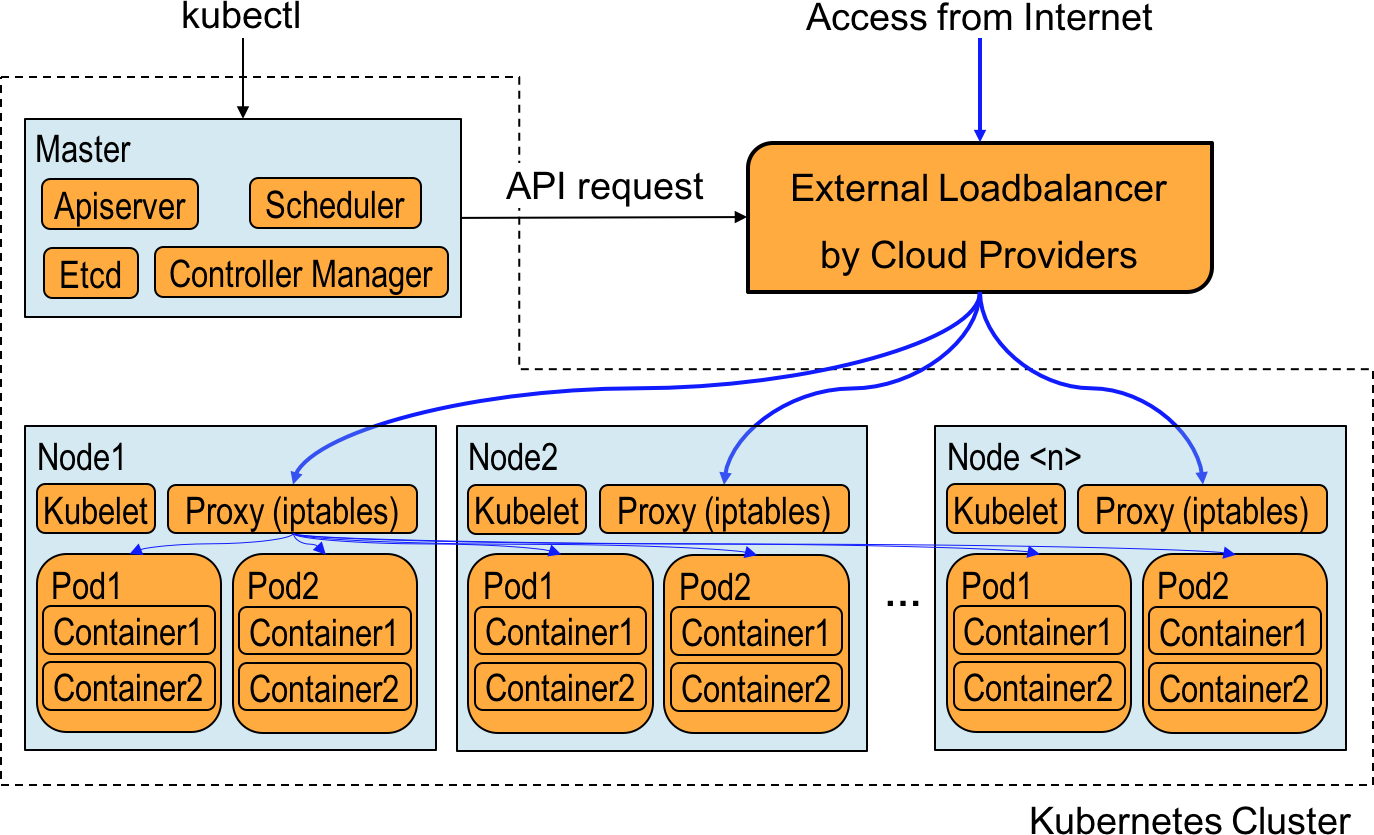
\includegraphics[width=\columnwidth]{Figs/K8sConventional}
\caption{Conventional architecture of a Kubernetes cluster.}
\label{fig:K8sConventional}
\end{figure}

Problems commonly occur when the Kubernetes container management system is used outside of recommended cloud providers(such as GCP or AWS).
Figure~\ref{fig:K8sConventional} shows an exemplified Kubernetes cluster.
A Kubernetes cluster typically consists of a master and nodes. They can be physical servers or VMs.
On the master, daemons that control the Kubernetes cluster are typically deployed. 
These daemons include, apiserver, scheduler, controller-manager and etcd. 
On the nodes, the kubelet daemon will run {\it pods}, depending the PodSpec information obtained from the apiserver on the master.
A {\em pod} is a group of containers that share same net name space and cgroups, 
and is the basic execution unit in a Kubernetes cluster.

When a service is created, the master will schedule where to run {\em pods} and kubelets on the nodes will launch them accordingly.
At the same time, the masters will send out requests to cloud provider API endpoints, asking them to set up external load balancers.
The proxy daemon on the nodes will also setup iptables DNAT\cite{MartinA.Brown2017} rules. 
The Internet traffic will then be evenly distributed by the external load balancer to nodes, 
after which it will be distributed again by the DNAT rules on the nodes to the designated {\em pods}. 
The returning packets will follow the exact same route as the incoming ones.

This architecture has the followings problems: 
1) Having external load balancers whose APIs are supported by the Kubernetes daemons is a prerequisite. 
There are numerous load balancers which is not supported by the Kubernetes.
These include the bare metal load balancers for on-premise data centers.  
In such cases, a user could manually setup the routing table on the gateway so that the traffic would be routed to one of the nodes.
Then the traffic would be distributed by the DNAT rules on the node to the designated {\em pods}.
However, this approach would require complicated network configuration and significantly degrade the portability of container clusters.
2) Distributing the traffic twice, first on the external load balancers and second on each node, 
complicates the administration of packet routing. 
Imagine a situation in which the DNAT table on one of the nodes malfunctions.
In such a case, only occasional timeouts would be observed, which would make it very difficult to find out which node was malfunctioning.   

In short, 1) Kubernetes can be used only in limited environments where the external load balancers are supported, 
and 2) the routes incoming traffic follow are very complex.

In order to address these problems, we propose a containerized software load balancer 
that is deployable in any environment even if there are no external load balancers.

\subsection{Proposed architecture}

\begin{figure}
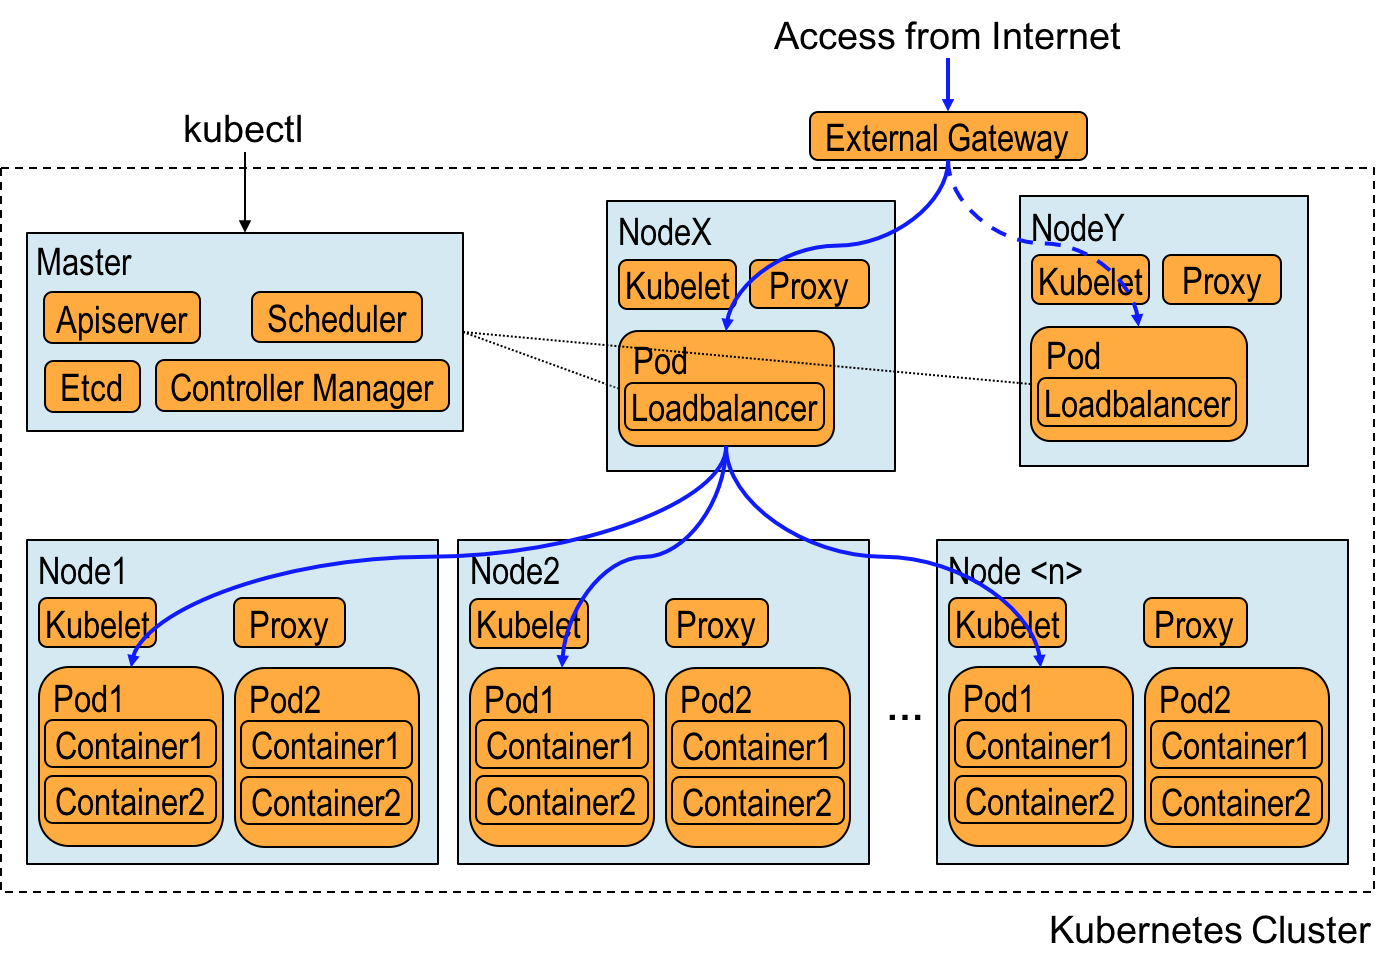
\includegraphics[width=\columnwidth]{Figs/K8sProposed}
\caption{Kubernetes cluster with proposed load balancer.}
\label{fig:K8sProposed}
\end{figure}

Figure~\ref{fig:K8sProposed} shows the proposed  Kubernetes cluster architecture, 
which has the following characteristics:
1) Each load balancer itself is run as a {\em pod} by Kubernetes. 
2) Load balancer configurations are dynamically updated based on information about running {\em pods}.
%%3) There exist multiple load balancers for redundancy. 
The proposed load balancer can resolve the conventional architecture problems, as follows:
Since the load balancer itself is containerized, load balancer can run in any environment including on-premise data centers, 
even without external load balancers that is supported by Kubernetes.
The incoming traffic is directly distributed to designated {\em pods} by the load balancer. 
It makes the administration, e.g. finding malfunctions, easier.

We designed the proposed load balancer using three components, IPVS, keepalived, and a controller. 
These components are placed in a Docker container image.
The IPVS is a Layer-4 load balancer capability, which is included in the Linux kernel 2.6.0 released in 2003 or later, 
to distribute incoming Transmission Control Protocol(TCP) traffic to 
{\em real servers}\footnote{The term, {\em real servers} refers to worker servers that will respond to incoming traffic, 
in the original literature\cite{Zhang2000}. We will also use this term in the similar way.}\cite{Zhang2000}. 
For example, IPVS distributes incoming Hypertext Transfer Protocol(HTTP) traffic destined for a single destination IP address, 
to multiple HTTP servers(e.g. Apache HTTP or nginx) running on multiple servers in order to improve the performance of web services.
Keepalived is a management program that performs health checking for {\em real servers}
and manage IPVS balancing rules in the kernel accordingly.
It is often used together with IPVS to facilitate ease of use.
Although keepalived also supports Virtual Router Redundancy Protocol(VRRP)\cite{hinden2004virtual}, the authors leave that topic for future work.
The controller is a daemon that periodically monitors the {\em pod} information on the master, 
and performs various actions when such information changes.
Kubernetes provides ingress controller framework as the Go Language(Golang) package to implement such controllers. 
We have implemented a controller program that will feed {\em pod} state changes to keepalived 
using this framework. 

These are the main ideas behind our proposal. In the following section, we will explain their implementation in detail.

\subsection{Implementation}\label{Implementation}

\begin{figure}
\includegraphics[width=\columnwidth]{Figs/IPVS-ingress-schem}
\caption{Implementation}
\label{fig:IPVS-ingress-schem}
\end{figure}

The proposed load balancer needs to dynamically reconfigure the IPVS balancing rules whenever {\em pods} are created/deleted. 
Figure~\ref{fig:IPVS-ingress-schem} is a schematic diagram to show the dynamic reconfiguration of the IPVS rules.
The right part of the figure shows the enlarged view of one of the nodes where the load balancer pod(LB2) is deployed.
Two daemon programs, controller and keepalived, run in the container inside the LB2 pod are illustrated.
The keepalived manages Linux kernel's IPVS rules depending on the ipvs.conf configuration file.
It is also capable of health-checking the liveliness of {\em real server}, 
which is represented as a combination of the IP addresses and port numbers of the target {\em pods}. 
If the health check to a {\em real server} fails, keepalived will remove that {\em real server} from the IPVS rules.

The controller monitors information concerning the running {\em pods} of a service 
in the Kubernetes cluster by consulting the apiserver running on the master.
Whenever {\em pods} are created or deleted, the controller will automatically regenerate an appropriate ipvs.conf 
and issue SIGHUP to keepalived.
Then, keepalived will reload the ipvs.conf and modify the kernel's IPVS rules accordingly.
The actual controller\cite{ktaka_ccmp_2017_826894} is implemented using the Kubernetes ingress controller\cite{K8sIngress2017} framework. 
By importing existing Golang package, \enquote{k8s.io/ingress /core/pkg/ingress}, we could simplify the implementation, e.g. 
120 lines of code.  

%In this way, the IPVS's balancing rules inside Linux kernel are maintained so that it can distribute the incoming traffic only to the living pods.

Configurations for capabilities were needed in the implementation: adding the CAP\_SYS\_MODULE capability 
to the container to allow the kernel to load required kernel modules inside a container, 
and adding CAP\_NET\_ADMIN capability to the container to allow keepalived to manipulate the kernel's IPVS rules. 
For the former case, we also needed to mount the \enquote{/lib/module} of the node's file system on the container's file system.

\begin{figure}
\begin{minipage}{0.7\columnwidth}
\begin{verbatim}
virtual_server fwmark 1 {
  delay_loop 5
  lb_algo lc
  lb_kind NAT
  protocol TCP
  real_server 172.16.21.2 80 {
    uthreshold 20000
    TCP_CHECK {
      connect_timeout 5
      connect_port 80
    }
  }
  real_server 172.16.80.2 80 {
    uthreshold 20000
    TCP_CHECK {
      connect_timeout 5
      connect_port 80
    }
  }
}
\end{verbatim}
\end{minipage}
\caption{An example of ipvs.conf}
\label{fig:ipvs.conf}
\end{figure}

\begin{figure}
\begin{minipage}{\columnwidth}
\small
\begin{verbatim}
# kubectl exec -it IPVS-controller-4117154712-kv633 -- IPVSadm -L
IP Virtual Server version 1.2.1 (size=4096)
Prot LocalAddress:Port Scheduler Flags
  -> RemoteAddress:Port Forward Weight ActiveConn InActConn
FWM  1 lc
  -> 172.16.21.2:80      Masq    1      0          0         
  -> 172.16.80.2:80      Masq    1      0          0
\end{verbatim}
\end{minipage}
\caption{Example of IPVS balancing rules}
\label{fig:IPVS rule}
\end{figure}


Figure~\ref{fig:ipvs.conf} and Figure~\ref{fig:IPVS rule} show an example of an ipvs.conf file 
generated by the controller and the corresponding IPVS load balancing rules, respectively.
Here, we can see that the packet with {\tt fwmark=1}\cite{BertHubert2002} is distributed 
to {\tt 172.16.21.2:80} and {\tt 172.16.80.2:80} 
using the masquerade mode(Masq) and 
the least connection(lc)\cite{Zhang2000} balancing algorithm.

\section{Performance measurement}\label{Performance Measurement}


We will now discuss the feasibility of the proposed load balancer by comparing 
its performance with those of existing iptables DNAT and the Nginx based load balancers. 
We conducted the performance measurements using the benchmark program called wrk\cite{Glozer2016}.

We also investigated the performance varying two network configurations: 
First one is an overlay network setting\cite{Sill2016,Marmol2015} that is often used to build the Kubernetes cluster. 
Flannel\cite{CoreOSFlannel} is one of popular overlay network technologies. 
We compared the performances of three backends settings\cite{CoreOSFlannelBackend}, 
{\it i.e.} operating modes of flannel, to find the best setting.
The other one is the setting for distributed packet processing.
It is well known that distributing handling of interrupts from the network interface card(NIC) 
and the subsequent IP protocol processing, among multiple cores impact the network performance.
In order to derive the best performance from load balancers, 
we also investigated how this setting would affect their performance.

The following subsections explain these in further detail. 

\subsection{Benchmark method}

\begin{figure}
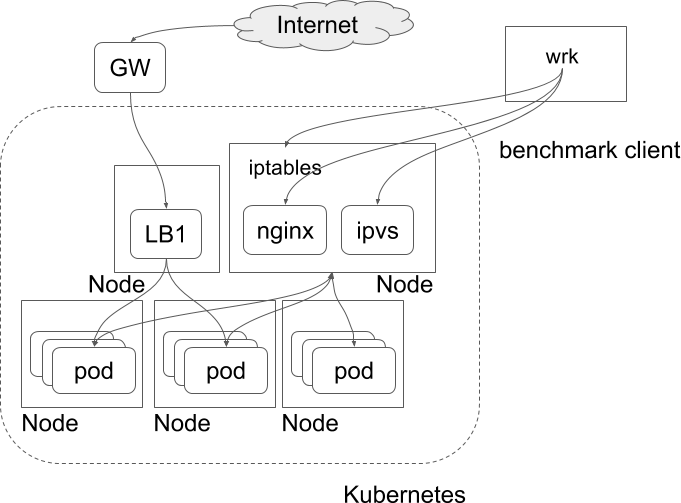
\includegraphics[width=\columnwidth]{Figs/benchmark-schem}
\caption{Benchmark setup}
\label{fig:benchmark-schem}
\end{figure}

We measured the performance of the load balancers using the wrk.
Figure~\ref{fig:benchmark-schem} illustrates a schematic diagram of our experimental setup.
Multiple {\em pods} are deployed on multiple nodes in the Kubernetes cluster. 
In each {\em pod}, a Nginx web server that returns the IP address of the {\em pod} are running.
We then set up the IPVS, iptables DNAT, and Nginx load balancers on one of the nodes(the top right node in the Figure~\ref{fig:benchmark-schem}). 

We measured the throughput, Request/sec, of the web service running on the Kubernetes cluster as follows:
The HTTP GET requests are sent out by the wrk on the client machine toward the nodes,
using destination IP addresses and port numbers that are chosen based on the type of the load balancer on which the measurement is performed.
The load balancer on the node then distributes the requests to the {\em pods}.
Each {\em pod} will return HTTP responses to the load balancer, after which the load balancer returns them to the client.
Based on the number of responses received by wrk on the client, 
load balancer performance, in terms of Request/sec can be obtained. 

Figure~\ref{fig:benchmark example} shows an example of the command-line for wrk and the corresponding output.
The command-line in Figure~\ref{fig:benchmark example} will generate 40 wrk program threads 
and allow those threads to send out a total of 800 concurrent HTTP requests over the period of 30 seconds.
The output example shows information including per thread statistics, error counts, Request/sec and Transfer/sec.

Figure~\ref{fig:Hardware and software configuration} shows hardware and software configuration used in our experiments.
We configured Nginx HTTP server to return a small HTTP content, 
the IP address of the {\em pod}, to make a relatively severe condition for load balancers. 
The size of the character string making up an IP address is limited to 15 bytes.
If we had chosen the HTTP response size so that most of the IP packet resulted in maximum transmission unit(MTU), 
the performance would have been limited by the Ethernet bandwidth.
However, since we used small HTTP responses, we could purely measure the load balancer performance.

The hardware we used had eight physical CPU cores and a NIC with 4 rx-queues.

\begin{figure}
\begin{minipage}{\columnwidth}
\small
\begin{Verbatim}[commandchars=\\\{\}]
\underline{\textbf{Command line:}}
 wrk -c800 -t40 -d30s http://172.16.72.2:8888/
-c: concurrency, -t: # of thread, -d: duration

\underline{\textbf{Output example:}}
 Running 30s test @ http://10.254.0.10:81/
  40 threads and 800 connections
  Thread Stats   Avg      Stdev     Max   +/- Stdev
    Latency    15.82ms   41.45ms   1.90s    91.90%
    Req/Sec     4.14k   342.26     6.45k    69.24%
  4958000 requests in 30.10s, 1.14GB read
  Socket errors: connect 0, read 0, write 0, timeout 1
Requests/sec: 164717.63
Transfer/sec:     38.86MB
\end{Verbatim}
\end{minipage}
\caption{Example output of benchmark by wrk}
\label{fig:benchmark example}
\end{figure}

\begin{figure}
\begin{minipage}{0.9\columnwidth}
\small
\begin{Verbatim}[commandchars=\\\{\}]
\underline{\textbf{Physical Machine Specification:}}
  CPU: Intel(R) Xeon(R) CPU E5-2450 0 @ 2.10GHz
  # of Physical Cores: 8
  Hyper Threading: enabled
  Memory: 32GB
  NIC: Broadcom BCM5720 Gigabit Ethernet PCIe

\underline{\textbf{Number of Physical Machines:}}
  Master: 1
  Node: 7
  Client: 1

\underline{\textbf{Node Software version:}}
  OS: Debian 8.7 (Jessie)
  Kernel: \footnotesize{3.16.0-4-amd64 #1 SMP Debian 3.16.39-1 (2016-12-30)}
  Kubernetes v1.5.2
  flannel v0.7.0
  etcd version: 3.0.15

\underline{\textbf{Load balancer Software version:}}
  Keepalived: v1.3.2 (12/03,2016)
  Nginx: nginx/1.11.1

\underline{\textbf{Worker Pod Software version:}}
  nginx : nginx/1.13.0 
\end{Verbatim}
\end{minipage}
\caption{Hardware and software configuration}
\label{fig:Hardware and software configuration}
\end{figure}


\subsection{Overlay network}

We used flannel to build the Kubernetes cluster used in our experiment.
Flannel has three types of backend, {\it i.e.}, operating modes, named host-gw, vxlan, and udp\cite{CoreOSFlannelBackend}.

In the host-gw mode, the flanneld installed on a node simply configures the routing table 
based on the IP address assignment information of the overlay network, which is stored in the etcd. 
When a {\em pod} on a node sends out an IP packet to {\em pods} on the different node, 
the former node consults the routing table and learn that the IP packet should be sent out to the latter.
Then, the former node forms Ethernet frames containing the destination MAC address of the latter node 
without changing the IP header, and send them out.

In the case of the vxlan mode, flanneld creates the Linux kernel's vxlan device, flannel.1. 
Flanneld will also configures the routing table appropriately based on the information stored in the etcd.
When {\em pods} on different nodes need to communicate, the packet is routed to flannel.1.
The vxlan functionality of the Linux kernel identify the MAC address of flannel.1 device on the destination node,
then form an Ethernet frame toward the MAC address.
The vxlan then encapsulates the Ethernet frame in a UDP/IP packet with a vxlan header, after which the IP packet is eventually sent out.

In the case of udp mode, flanneld creates the tun device, flannel0, and configures the routing table.
The flannel0 device is connected to the flanneld daemon itself.
An IP packet routed to flannel0 is encapsulated by flanneld, and eventually sent out 
to the appropriate node. 
The encapsulation is done for IP packets.

Figure~\ref{fig:flannel-packet-diagram} shows the schematic diagrams of frame formats for three backends modes of the flannel overlay network. 
The MTU sizes in the backends, assuming the MTU size without encapsulation is 1500 bytes, are also presented.
Since packets are not encapsulated in the host-gw mode, the MTU size remains 1500 bytes.
An additional 50 bytes of header is used in the vxlan mode, thereby resulting in an MTU size of 1450 bytes.
In the case of the udp mode, only 28 bytes of header are used for encapsulation, which results in an MTU size of 1472 bytes.

\begin{figure}
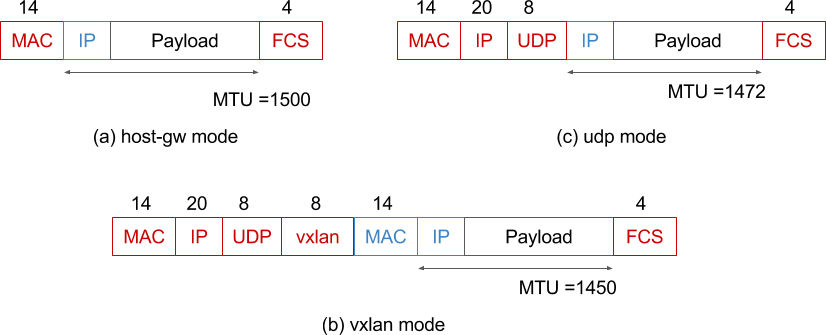
\includegraphics[width=\columnwidth]{Figs/flannel-packet-diagram}
\caption{frame diagram}
\label{fig:flannel-packet-diagram}
\end{figure}

Performance of the load balancers can be influenced by the overhead of encapsulation. 
Thus, the host-gw mode, where there is no overhead due to encapsulation, 
results in the best performance levels as shown in Section~\ref{Result and Discussion}.
However, the host-gw mode has a significant drawback that prohibit it to work correctly in cloud platforms. 
Since the host-gw mode simply sends out a packet without encapsulation, if there is a cloud gateway between nodes, 
the gateway cannot identify the proper destination, thus drop the packet.

\begin{table}
  \begin{tabular}{lccc}
    \toprule
    flannel backend & On-premise & GCP & AWS \\
    \midrule
    host-gw & OK & NG & (OK) \\
    vxlan & OK & OK & OK \\
    udp & OK & OK & OK \\
    \bottomrule
\end{tabular}

  \caption{Viable flannel backend modes}
  \label{tab:Viable flannel backends}
\end{table}

We conducted an investigation to determine which of the flannel backend mode would be usable on AWS, GCP, and on-premise data centers.
The results are summarized in Table~\ref{tab:Viable flannel backends}. 
In the case of GCP, an IP address of {\tt /32} is assigned to every VM host and 
every communication between VMs goes through GCP's gateway.
As for AWS, the VMs within the same subnet communicate directly, while the VMs in different subnets communicate via the AWS's gateway.
Since the  gateways do not have knowledge of the flannel overlay network, they drop the packets; thereby, 
they prohibit the use of the flannel host-gw mode in those cloud providers.  

In our experiment, we compared the performance of load balancers when different flannel backend modes were used. 

\subsection{Distributed packet handling}

Recently, the performance of CPUs are improved significantly due to the development of multi-core CPUs.
One of the top of the line server processors from Intel now includes up to 28 cores in a single CPU.
In order to enjoy the benefits of multi-core CPUs in communication performance, 
it is necessary to distribute the handling of interrupts from the NIC and the IP protocol processing
to the available physical cores.
Receive Side Scaling (RSS)\cite{TomHerbert} is a technology 
to distribute handling of the interrupt from NIC queues to multiple CPU cores.
Subsequently, Receive Packet Steering (RPS)\cite{TomHerbert} distributes the IP protocol processing 
to multiple CPU cores by issuing inter core software interrupts.

Since load balancer performance levels could be affected by these technologies,
we conducted an experiment to determine how load balancer performance level change depending on the RSS and RPS settings.
The following shows how RSS and RPS are enabled and disabled in our experiment. 
The NIC used in our experiment is Broadcom BCM5720, which has four rx-queues and one tx-queue.
Figure~\ref{fig:rx-queue} shows the interrupt request (IRQ) number assignments to those NIC queues.

\begin{figure}
%\begin{center}
\begin{minipage}{0.7\columnwidth}
\small
\begin{verbatim}
81: eth0-tx-0
82: eth0-rx-1
83: eth0-rx-2
84: eth0-rx-3
85: eth0-rx-4
# obtained from /proc/interrupts 
\end{verbatim}
\end{minipage}
\caption{RX/TX queues of the hardware}
\label{fig:rx-queue}
%\end{center}
\end{figure}

When packets arrive, they are distributed to these rx-queues depending on the flow each packet belongs to.
Each receive queue has a separate IRQ associated with it. The NIC triggers
this to notify a CPU when new packets arrive on the given queue.
Then, the notified CPU handles the interrupt, and performs the protocol processing. 
According to the \cite{TomHerbert}, the CPU cores allowed to be notified is controlled by setting 
a hexadecimal value corresponding to the bit maps indicating the allowed CPU cores in \enquote{/proc/irq/\$irq\_number /smp\_affinity}.
%
For example, in order to route the interrupt for eth0-rx-1 to CPU0, 
we should set \enquote{/proc/irq/82/smp\_affinity} 
to binary number {\tt 0001}, which is 1 in hexadecimal value.
Further, in order to route the interrupt for eth0-rx-2 to CPU1, we 
should set \enquote{/proc/irq/83/smp\_affinity} 
to binary number {\tt 0010}, which is 2 in hexadecimal value.

We refer the setting to distribute interrupts from four rx-queues to CPU0, CPU1, CPU2 and CPU3 as {\tt RSS = on}. 
It is configured as the following setting: 

\begin{center}
\begin{minipage}{0.8\columnwidth}
\begin{Verbatim}[commandchars=\\\{\}]

\underline{\textbf{RSS=on}}
echo 1 > /proc/irq/82/smp_affinity
echo 2 > /proc/irq/83/smp_affinity
echo 4 > /proc/irq/84/smp_affinity
echo 8 > /proc/irq/85/smp_affinity

\end{Verbatim}
\end{minipage}
\end{center}

On the other hand, {\tt RSS = off} means that an interrupt from any rx-queue is routed to CPU0. 
It is configured as the following setting:

\begin{center}
\begin{minipage}{0.8\columnwidth}
\begin{Verbatim}[commandchars=\\\{\}]

\underline{\textbf{RSS=off}}
echo 1 > /proc/irq/82/smp_affinity
echo 1 > /proc/irq/83/smp_affinity
echo 1 > /proc/irq/84/smp_affinity
echo 1 > /proc/irq/85/smp_affinity

\end{Verbatim}
\end{minipage}
\end{center}

%In this case, interrupt from any of rx-queue is routed to CPU0.

The RPS distributes IP protocol processing by placing the packet
on the desired CPU's backlog queue and wakes up the CPU using inter-processor interrupts.
We have used the following settings to enable the RPS:

\begin{center}
\begin{minipage}{0.95\columnwidth}
\begin{Verbatim}[commandchars=\\\{\}]

\underline{\textbf{RPS=on}}
echo fefe > /sys/class/net/eth0/queues/rx-0/RPS_cpus
echo fefe > /sys/class/net/eth0/queues/rx-1/RPS_cpus
echo fefe > /sys/class/net/eth0/queues/rx-2/RPS_cpus
echo fefe > /sys/class/net/eth0/queues/rx-3/RPS_cpus

\end{Verbatim}
\end{minipage}
\end{center}

Since the hexadecimal value \enquote{fefe} represented as \enquote{1111 1110 1111 1110} in binary, 
this setting will allow distributing protocol processing to all of the CPUs, except for CPU0 and CPU8.
In this paper, we will refer this setting as {\tt RPS = on}.
%
On the other hand, {\tt RPS = off} means that no CPU is allowed for RPS. 
Here, the IP protocol processing is performed on the CPUs the initial hardware interrupt is received.
It is configured as the following settings:

\begin{center}
\begin{minipage}{0.9\columnwidth}
\begin{Verbatim}[commandchars=\\\{\}]

\underline{\textbf{RPS=off}}
echo 0 > /sys/class/net/eth0/queues/rx-0/RPS_cpus
echo 0 > /sys/class/net/eth0/queues/rx-1/RPS_cpus
echo 0 > /sys/class/net/eth0/queues/rx-2/RPS_cpus
echo 0 > /sys/class/net/eth0/queues/rx-3/RPS_cpus

\end{Verbatim}
\end{minipage}
\end{center}

The RPS is especially effective when the NIC does not have multiple receive queues or when the number of queues is 
much smaller than the number of CPU cores. 
That was the case of our experiment, where we had a NIC with only four rx-queues, 
while there was a CPU with eight physical cores.

\section{Result and Discussion}\label{Result and Discussion}

\begin{figure}
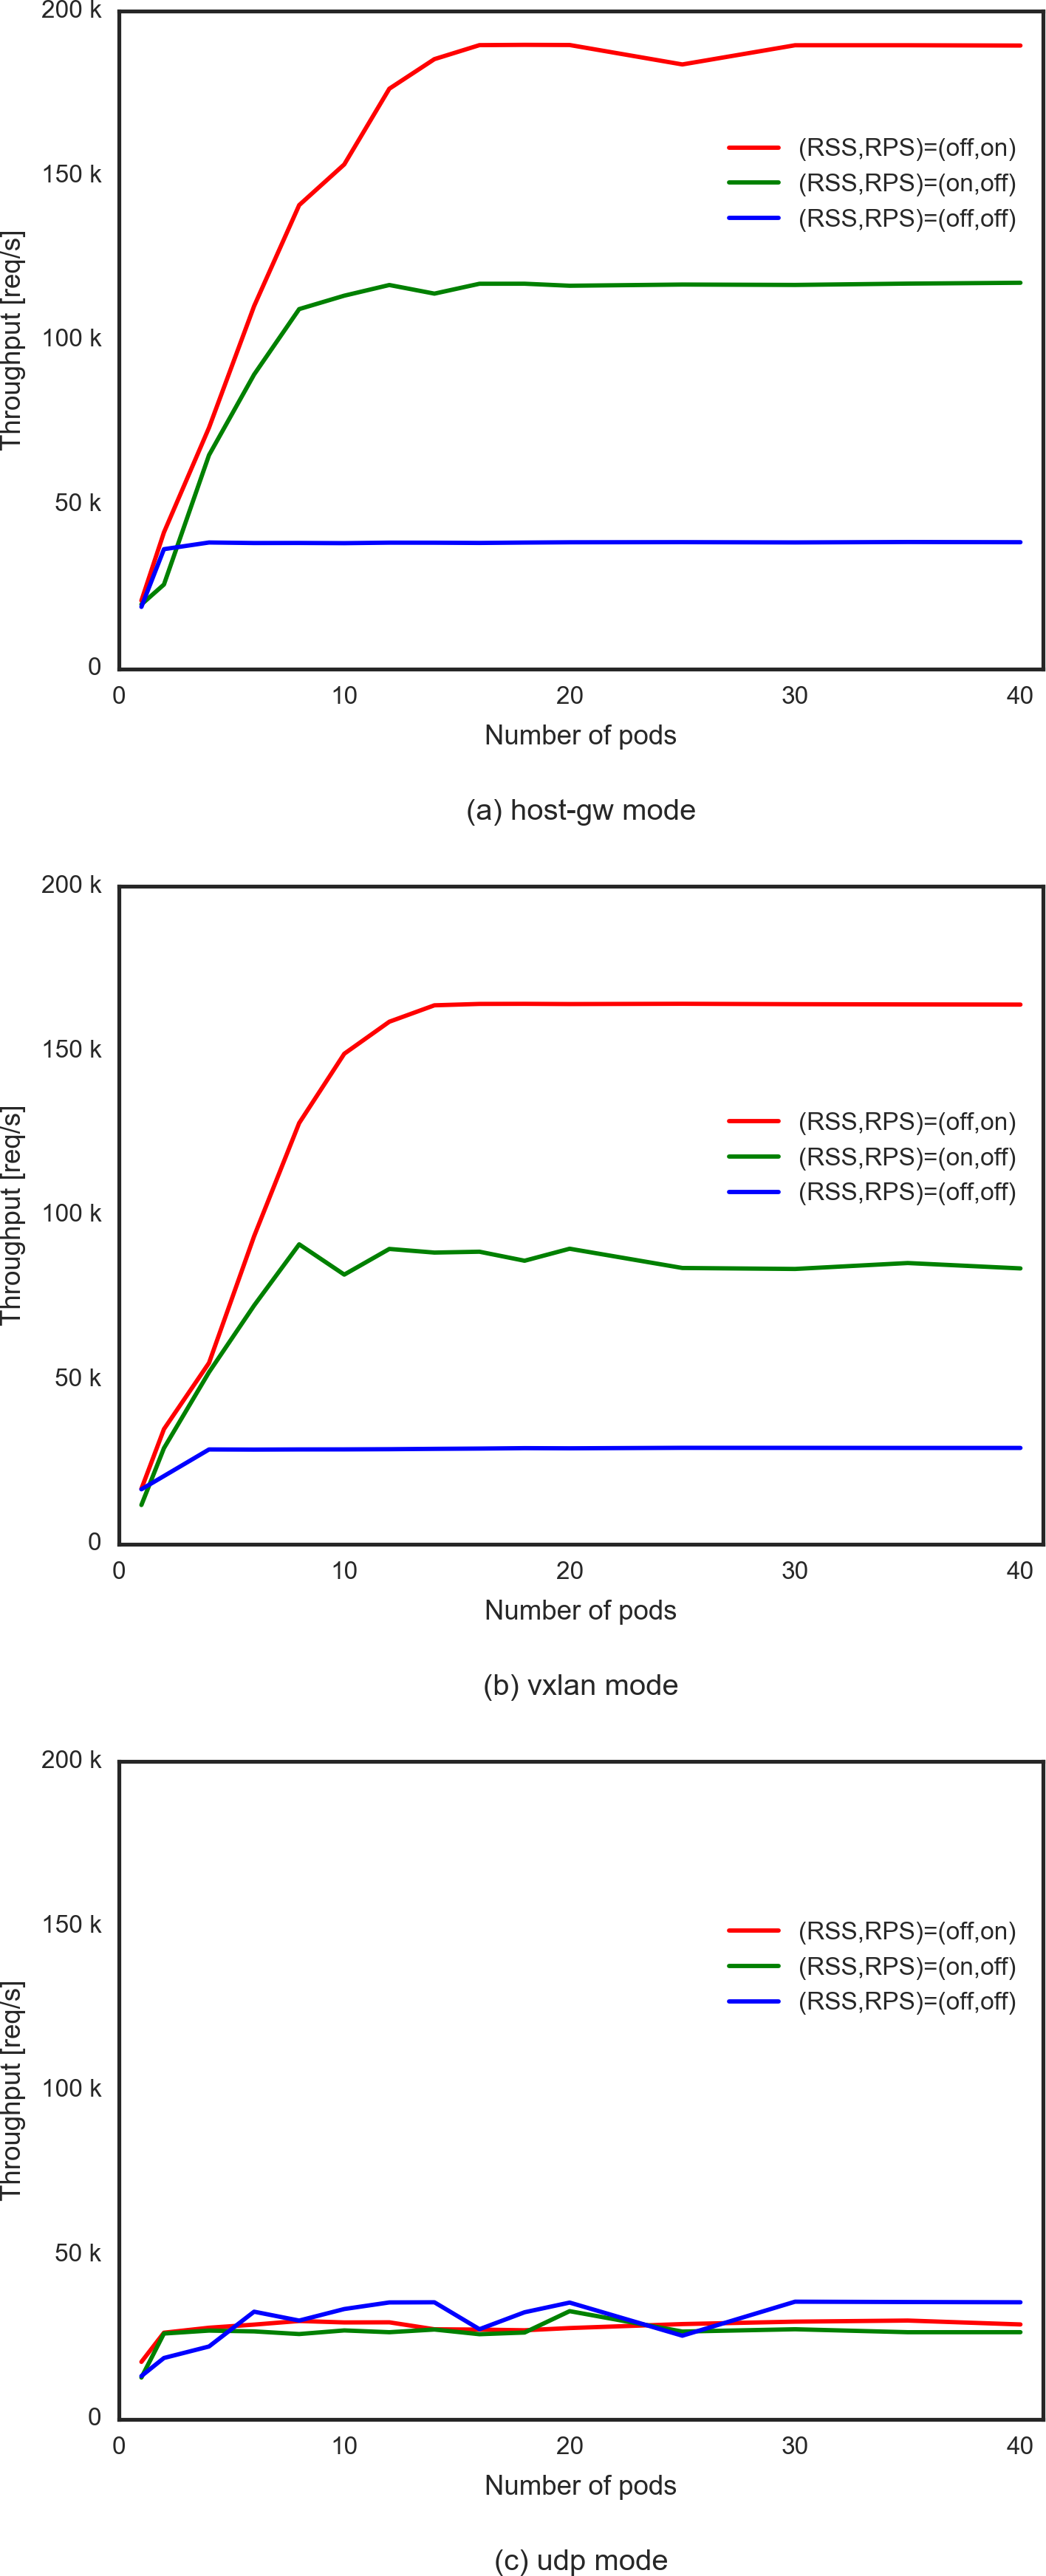
\includegraphics[width=\columnwidth]{Figs/ipvs_3figs}
\caption{IPVS results}
\label{fig:IPVS3figs}
\end{figure}

\begin{figure}
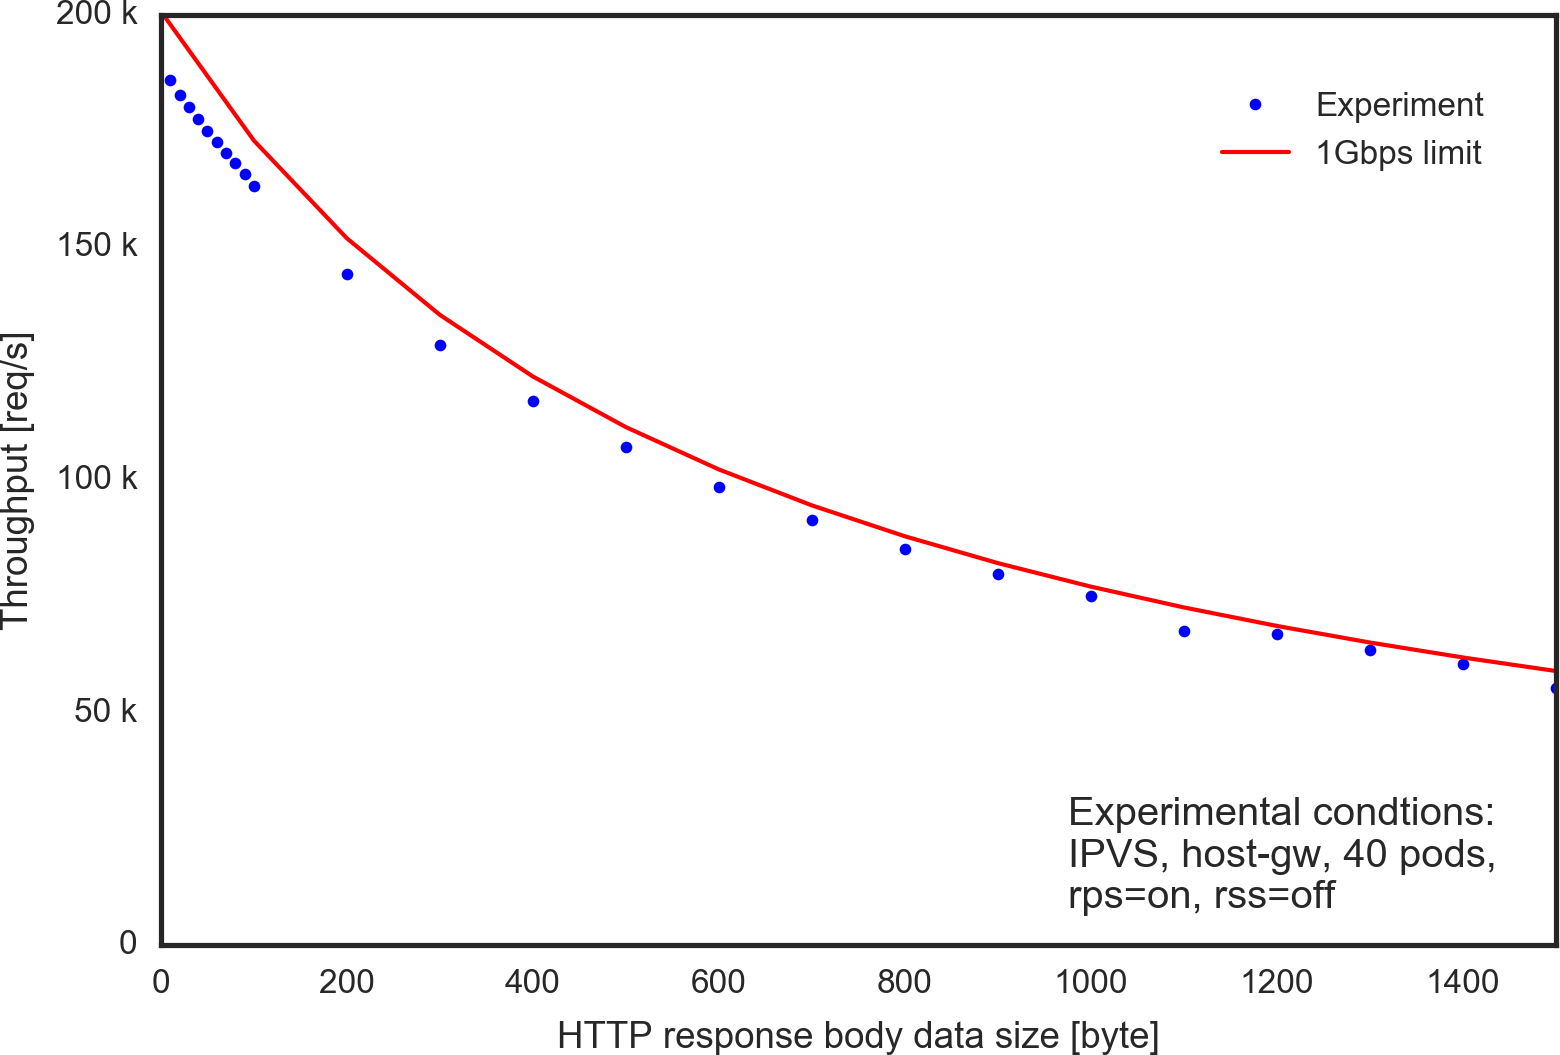
\includegraphics[width=\columnwidth]{Figs/performance_limitation}
\caption{Performance limitation due to 1Gbps bandwidth}
\label{fig:performance_limitation}
\end{figure}

\begin{figure}
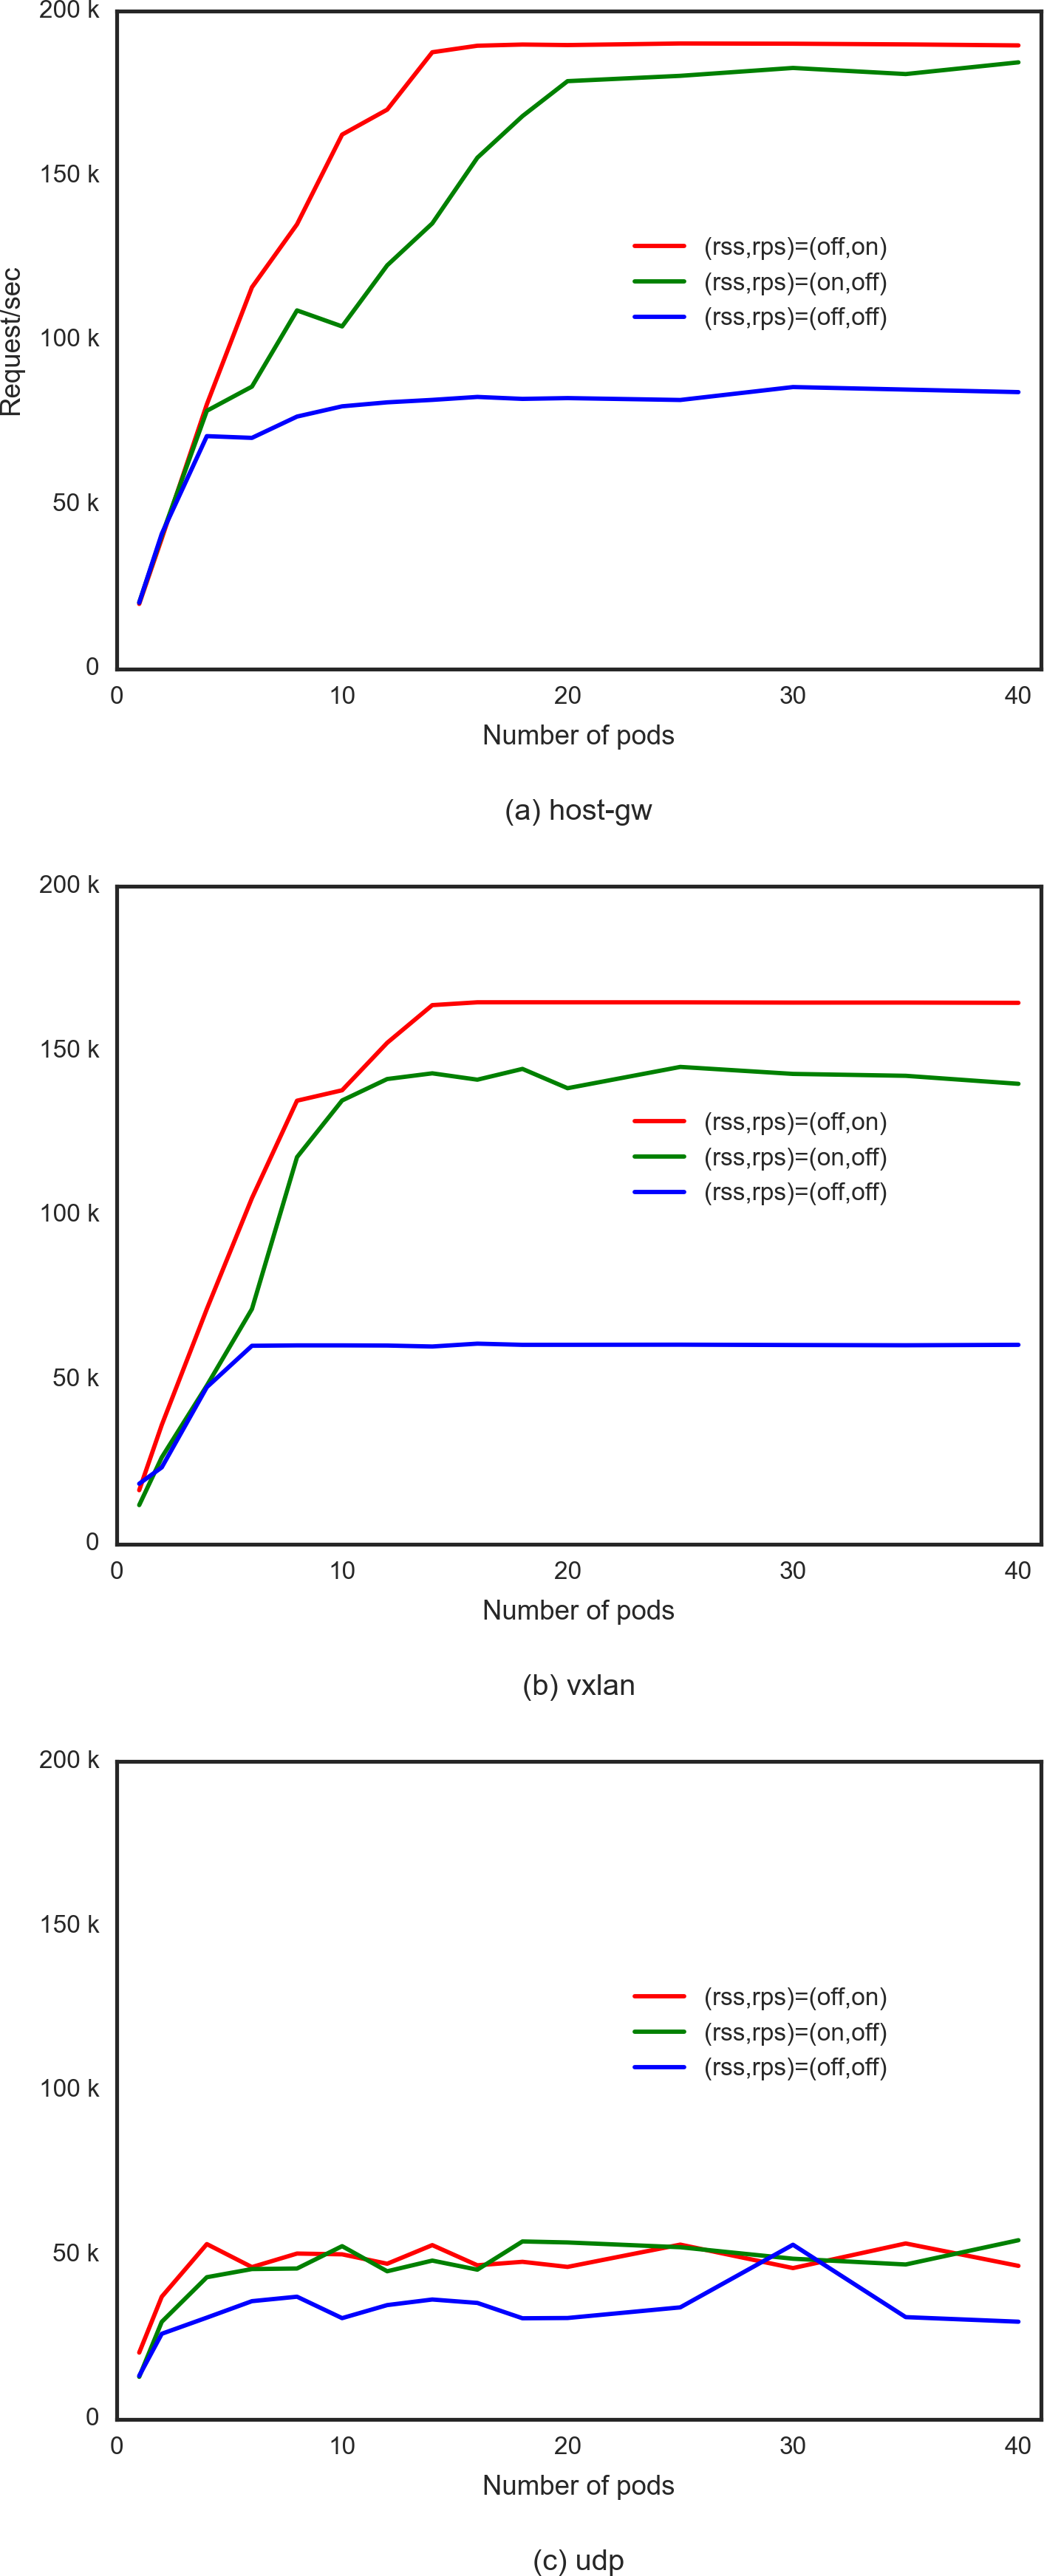
\includegraphics[width=\columnwidth]{Figs/iptables_3figs}
\caption{iptables results}
\label{fig:iptabls3figs}
\end{figure}

\begin{figure}
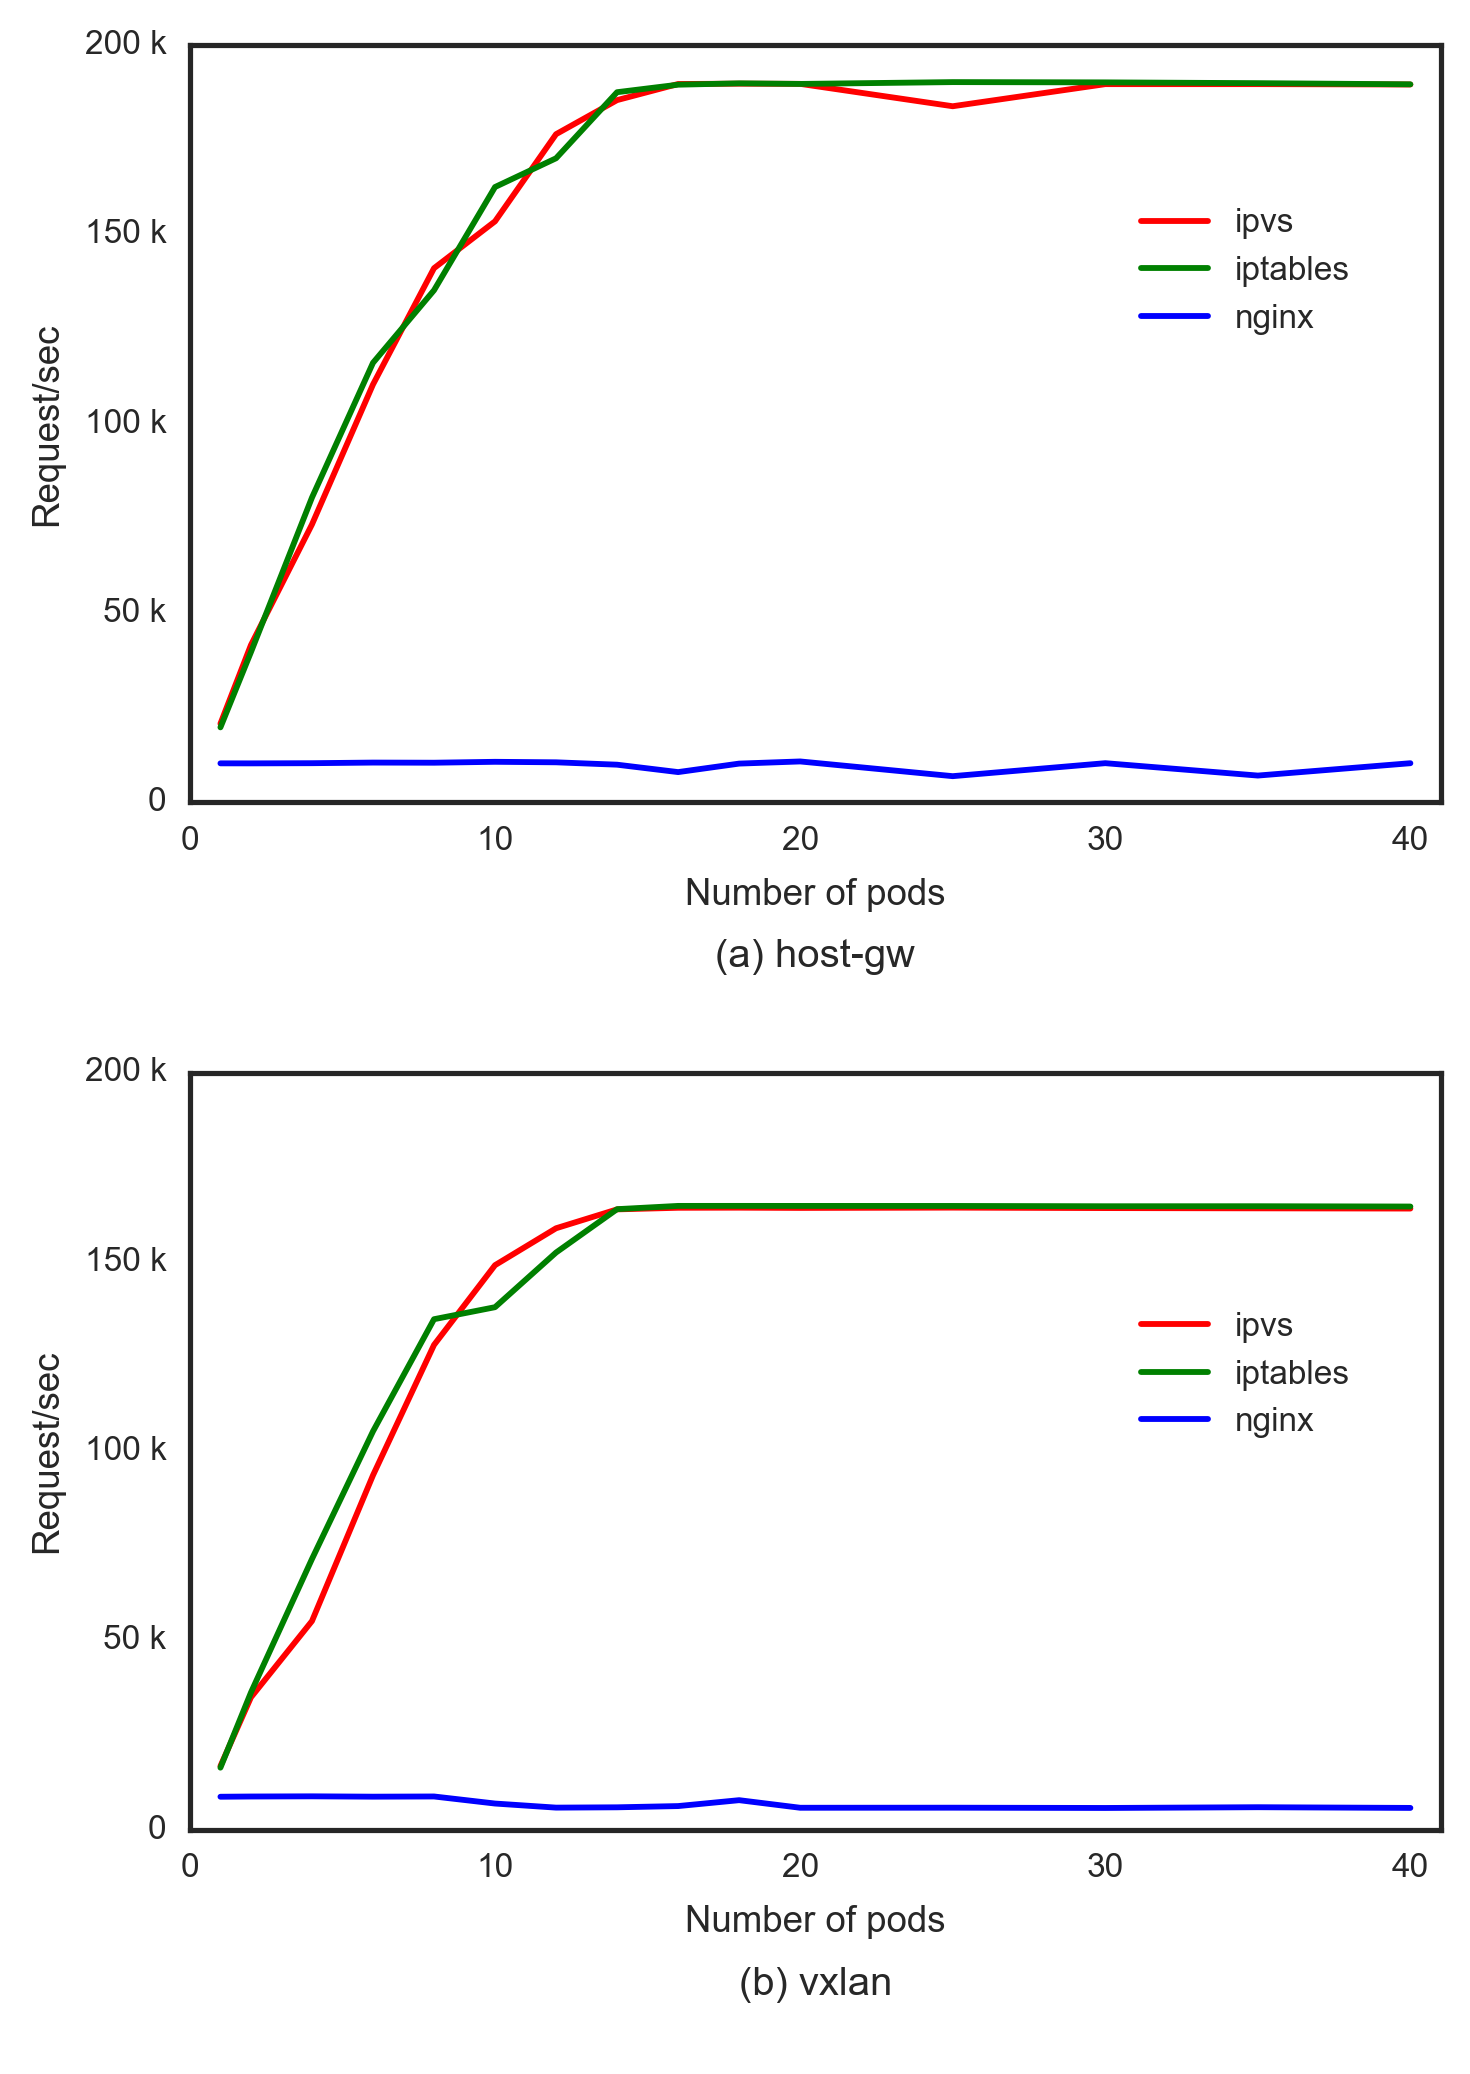
\includegraphics[width=\columnwidth]{Figs/ipvs-iptables-nginx_2figs}
\caption{IPVS and iptables comparison}
\label{fig:IPVS-iptables-nginx_2figs}
\end{figure}

\begin{figure}
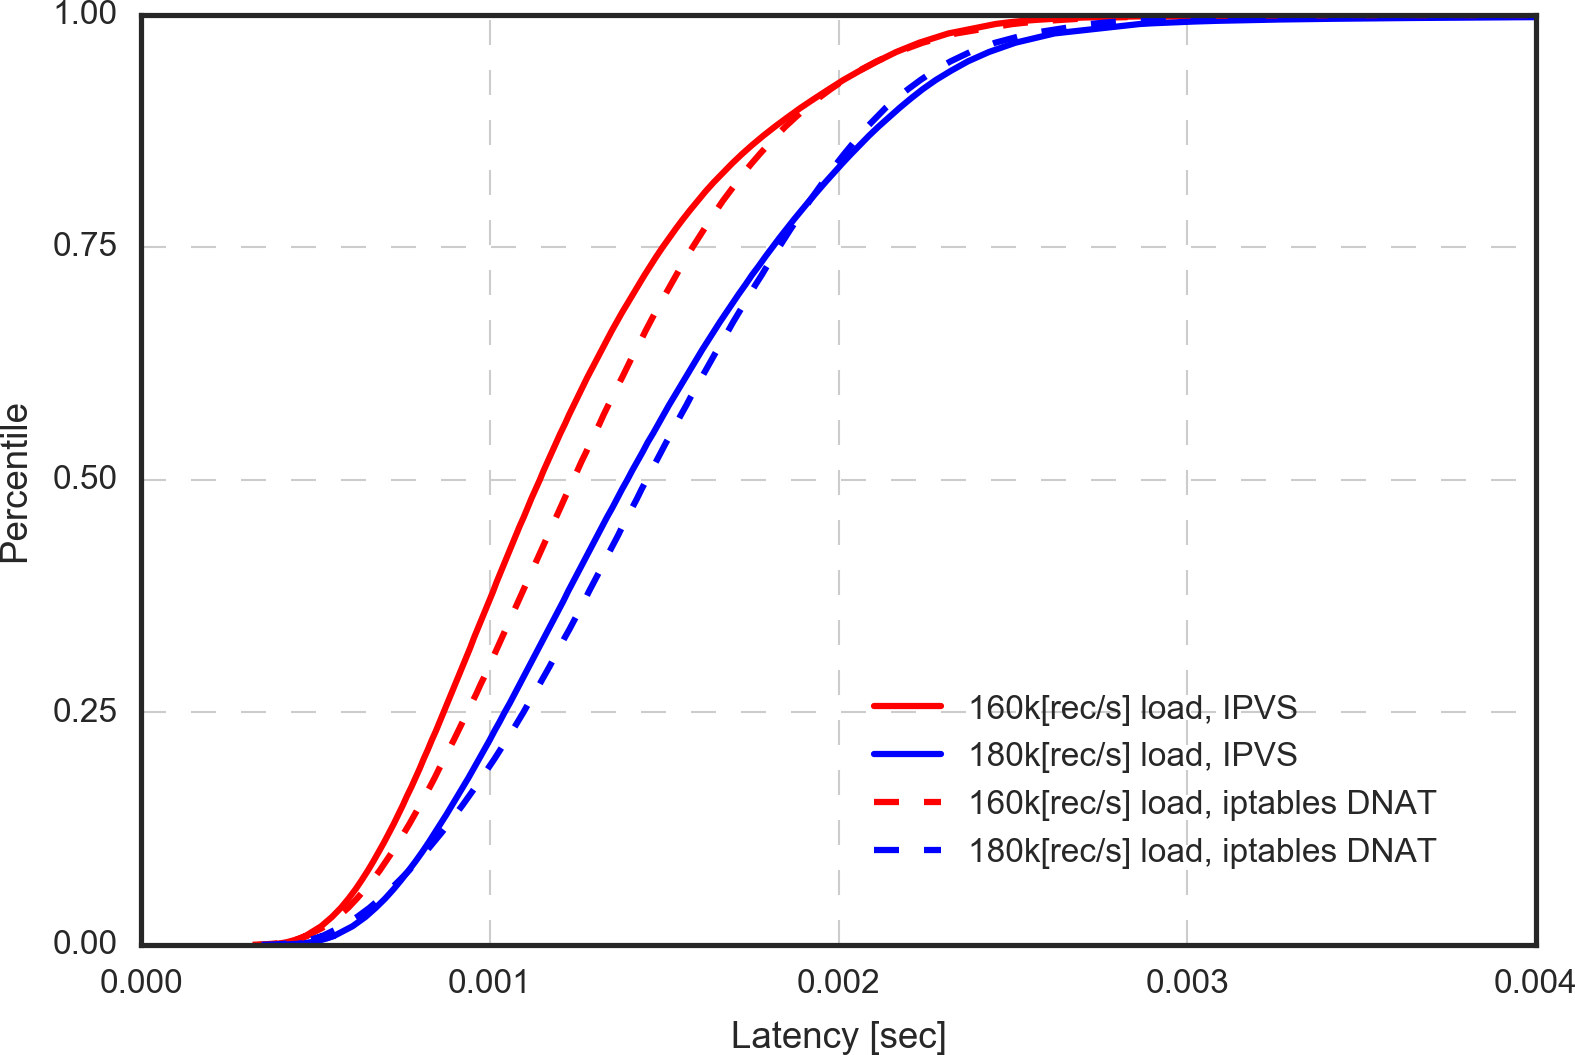
\includegraphics[width=\columnwidth]{Figs/latency_cdf_rps_40pods}
\caption{Latency CDF for 40 pods where flannel mode=host-gw, rps=on, rss=off}
\label{fig:latency_cdf_rps_40pods}
\end{figure}


Figure~\ref{fig:IPVS3figs} shows the IPVS load balancer performance, that is, 
the throughput (Request/sec) of the Nginx web server {\em pods} in our experiments.
As for the overlay network, we measured the performance for three flannel backend modes, 
host-gw (Figure~\ref{fig:IPVS3figs}(a)), vxlan (Figure~\ref{fig:IPVS3figs}(b)) and udp (Figure~\ref{fig:IPVS3figs}(c)).
The following RSS and RPS setting were compared: 

\begin{center}
\begin{minipage}{0.8\columnwidth}
\begin{verbatim}
(RSS, RPS) = (off, off)
           = (on , off)
           = (off, on )
\end{verbatim}
\end{minipage}
\end{center}

Except for the udp cases, we can see the trend in which the throughput linearly increases 
as the {\em pod} number increases and then it eventually saturates.
The saturated performance levels indicates the maximum performance of the IPVS load balancer.
The maximum performance limits depend on the flannel backend mode type and the (RSS, RPS) settings.
From the results in Figures~\ref{fig:IPVS3figs}(a,b), it can be seen that if we turn off distributed packet processing,
{\it i.e.}, when \enquote{(RSS, RPS) = (off, off)}, performance degrades significantly. 
In this case, the performance bottleneck is primarily due to packet processing in a single core.

If we compare the results for the cases when \enquote{(RSS, RPS) = (on, off)} and \enquote{(RSS, RPS) = (off, on)},
the latter is better than the former.
This is understandable, since in the case of \enquote{RPS = on}, eight physical cores can be used whereas 
in the case of \enquote{RSS = on} only four cores can be used, on the hardware used in our experiment.
The performance bottleneck of the case when \enquote{RSS = on} is considered 
to be due to the fact that the packet processing is only done on four CPU cores.
%
At first, it was not clear what caused the performance limit for the case when \enquote{RPS = on},
however we now suspect this is due to 1Gbps bandwidth limitation.
A packet level analysis using tcpdump\cite{jacobson1989tcpdump} revealed that 622.72 byte of extra HTTP headers, 
TCP/IP headers and ethernet frames are needed for each request in the case of the wrk benchmack program.  
This results in the upper limitation of 196,627 [req/s], where the date size of HTTP response body is 13 byte, or typical data size in our experiment. 
Figure~\ref{fig:performance_limitation} shows upper limitation of the performance level for 1Gbps ethernet together with 
actual benchmark results and we can conclude that when \enquote{RPS = on}, IPVS performance is limited by bandwidth.

If we compare the performances among the flannel backend modes types, 
the host-gw mode where no encapsulation is conducted shows the highest performance level,
followed by the vxlan mode where the Linux kernel encapsulate the Ethernet frame.
The udp mode where flanneld itself encapsulate the IP packet shows significantly lower performances levels.

Figure~\ref{fig:iptabls3figs} shows the performance of the load balancer 
functionality of the iptables DNAT. 
As can be seen in the figure, the performance value increases as the number of the {\em pod} increases linearly, 
and then becomes saturated at some point, as was the case with the IPVS results.

If we compare the results for different packet handling settings, the highest performance is 
obtained for the case when \enquote{(RSS, RPS) = (off on)}, followed by the case when \enquote{(RSS, RPS) = (on, off)}. 
The performance result for the case when \enquote{(RSS, RPS) = (off, off)} resulted in the 
poorest performance level, as was the case for the IPVS.
As for the flannel backend modes, the host-gw shows the highest performance followed 
by the vxlan. The udp backend mode totally degrades the performance level.

Figure~\ref{fig:IPVS-iptables-nginx_2figs} compares the performance measurement results 
among the IPVS, iptables DNAT, and Nginx load balancers
with the condition of \enquote{(RSS, RPS) = (off on)}.
The proposed IPVS load balancer exhibits almost equivalent performance as the existing iptables DNAT based load balancer. 
The Nginx based load balancer shows no performance improvement even though the number of the Nginx web server {\em pods} is increased.
It is understandable because the performance of the Nginx as a load balancer is expected to be similar to the performance as a web server.
Figure~\ref{fig:latency_cdf_rps_40pods} compares Cumulative Distribution Function(CDF) of the load balancer latency at the constant load.
The latencies are a little bit smaller for IPVS, however we consider the difference almost negligible.
For example, the median value at 160K[req/s] load for IPVS and iptables DNAT are, 1.1 msec and 1.2 msec, respectively.

\section{Conclusions}\label{Conclusions}

In this paper, we proposed a portable load balancer for the Kubernetes cluster systems 
that is aimed at facilitating migration of container clusters for web services.
We implemented a containerized software load balancer that is run by Kubernetes as a part of container cluster, 
using Linux kernel's IPVS, as a proof of concept.
In order to discuss the feasibility of the proposed load balancer, we built 
a Kubernetes cluster system and conducted performance measurements.
Our experimental results indicate that the IPVS based load balancer in container improves the portability of 
the Kubernetes cluster system while it shows the similar performance levels as the existing iptables DNAT based load balancer.
We also clarified that choosing the right operating modes of overlay networks is important for the performance of load balancers. 
For example, in the case of flannel, only the vxlan and udp backend operation modes could be used 
in the cloud environment, and the udp backend significantly degraded their performance.
Furthermore, we also learned that the distribution of packet processing among multiple CPUs was very important
to obtain the maximum performance levels from load balancers.
%

The limitations of this work that authors aware of include the followings; 
1) We have not discussed the load balancer redundancy. 
Routing traffic to one of the load balancers while keeping redundancy in the container environment is a complex issue,
because standard Layer 2 rendandacy protocols, VRRP or OSPF\cite{moy1997ospf} that uses multicast, can not be used in many cases.
Further more, providing uniform methods independent of various cloud environments and on premise datacenter is much more difficult.   
2) Experiments are conducted only in a 1Gbps network environment.
The experimental results indicate the performance of IPVS may be limited by the network bandwidth, 1Gbps, in our experiments. 
Thus, experiments with the faster network setting, e.g. 10Gigabit ethernet, are needed to investigate the feasibility of the proposed load balancer.
3) We have not yet compared the performance level of proposed load balance with those of cloud provider's load balancers.
It shoud be fair to compare the performance of proposed load balancer with those of the combination of the cloud load balancer and the iptables DNAT. 
The authors leave these issues for future work and they will be discussed elsewhere.

%\end{document}  % This is where a 'short' article might terminate


%\begin{acks}
%  The authors would like to thank lots of people.

%\end{acks}
